\subsection{Motivation} 

Today, the full exploitation of the lightweight potential of fibre reinforced plastics (FRP) is limited due to missing reliability of failure predictions of real structures, especially when taking into account determining manufacturing conditions. The underlying goal behind this study is to increase the understanding of failure mechanisms in FRP as shown in \autoref{fig:Exp:Failure} and their numerical simulation.

\begin{figure}[htbp]
  \begin{subfigure}{0.59\linewidth}
    \centering
    %\includegraphics[width=\linewidth, height=4cm,keepaspectratio]{../../Material/Figures/AFP-C-Gu-4-nB-v_by_Falk.jpg}
    \includegraphics[width=\linewidth, height=4cm,keepaspectratio]{AFP-C-Gu-4-nB-v_by_Falk.jpg}
    \caption{Crack in a CFRP specimen. Courtesy of DLR.}
    \label{fig:Exp:CompositeCrack}
  \end{subfigure}%
  \hfill
  \begin{subfigure}{0.39\linewidth}
    \centering
    %\includegraphics[width=\linewidth,height=4cm,keepaspectratio]{../../Material/Figures/Exp_Matrix_Failure}
    \includegraphics[width=\linewidth,height=4cm,keepaspectratio]{Exp_Matrix_Failure}
    \caption{Matrix failure \cite{GamstedtEK1999,KrauseD2016}}
    \label{fig:Exp:MatrixFailure}
  \end{subfigure}%
  \caption{Exemplary failure mechanisms in FRP materials}
  \label{fig:Exp:Failure}
\end{figure}

The current state-of-the-art methods used in industry and research for failure predictions are based on continuum mechanics (CM) and its numerical implementation in the finite element method (FEM). The continuum mechanics is well suited for stress analyses of undamaged structures, but it is unable to proper model damage evolution after initiation. The basic continuum mechanical theory was originally developed around 1822 by Augustin-Louis Cauchy  \cite{BobaruF2017}. The assumptions made by Cauchy lead to a mathematical description of continuous media partial differential equations (PDE). With proper restrictions, the PDEs are elliptic in equilibrium problems. It is to be noted that the underlying boundary value problems are generally well-posed for typical materials \cite{BobaruF2017}. This  made the PDEs solvable even in the pre-computer time. In reality, all materials are discontinuous and heterogeneous. For several problems, the usual assumption that at macroscopic length scales a material can be well approximated as continuous, is not valid. Obviously, a fracture in any material fails to satisfy the smoothness requirement.

To overcome this deficit, additional theories such as fracture mechanics are required and applied. However, certain levels of inconsistencies within the mathematical assumptions between continuum and fracture mechanics still lead to inaccurate damage prediction. Motivated by ideas of molecular dynamics, Stewart Silling developed the fundamental peridynamic theory in the early 2000's as an alternative theory to state-of-the-art modelling approaches \cite{SillingSA2000}. In this theory the fundamental PDE of the momentum conservation is replaced by an integral equation.
% This means, that all material within a finite distance, the horizon $\delta$, interact with each other.

Peridynamics (PD) presents a promising approach to simulate damage initiation, evolution and interaction in any material in one holistic approach. It is a non-local theory which takes long-range forces between material points in a certain neighborhood, the horizon $\delta$, into account. Constitutive models in peridynamics depend on finite deformation vectors, as opposed to classical constitutive models which depend on deformation gradients \cite{SelesonP2016}. In contrast to the FEM based on continuum mechanics, the peridynamic governing equations are based on integral equations, which are valid everywhere - whether a discontinuity exists in the material or not. Damage is directly incorporated in the material response.

% In this paper the peridynamic is utilized for ....
% 
% This stochastic analysis is used to determine a non-numerical dependent damage initiation mechanism?! Damage should be initiated by minor unsymmetries of the material and not by the distribution of the peridynamic bonds.
% The paper is structured as following. First the theoretical background of Peridynamics and the probabilistic analysis is illustrated. Second the models are described. Third the results are discussed and the paper is concluded.